\documentclass[a4paper]{report}
\usepackage[utf8]{inputenc}
\usepackage[spanish]{babel}
\usepackage[dvipsnames]{xcolor}
\usepackage{parskip}
\usepackage[colorlinks=true,urlcolor=blue,linkcolor=black]{hyperref}
\usepackage{url}
\usepackage{booktabs}
\usepackage{float}
\usepackage{adjustbox}
\usepackage{amsmath,amssymb}
\usepackage{graphicx}
\usepackage{geometry}
\usepackage{subfig}
\usepackage{caption}
\usepackage{wrapfig}
\usepackage{float}
\usepackage{multicol}
\usepackage{tcolorbox}
\usepackage{fancyvrb}
\usepackage{booktabs}
\usepackage{multirow}
\usepackage{lmodern}
\usepackage{color,array}
\usepackage{etoolbox}
\usepackage{minted}

\makeatletter
\patchcmd{\@makechapterhead}{\vspace*{50\p@}}{}{}{}% Removes space above \chapter head
\patchcmd{\@makeschapterhead}{\vspace*{50\p@}}{}{}{}% Removes space above \chapter* head
\makeatother

\unaccentedoperators

\setlength{\textfloatsep}{0pt}
\counterwithout{section}{chapter}

\title{\Huge{}\texttt{MIPS R2000}\\\vspace{8pt}\Large{}\textbf{\scalebox{.85}[1.0]{Práctica 1}}}
\author{Ariel Leonardo Fideleff}

\begin{document}

\pagenumbering{gobble}
\maketitle

\chapter{Cuestiones}

\section{Apartado 1}

\begin{center}
\large\textbf{-- \textsl{Declaración de palabras en memoria} --}
\end{center}

\subsection*{1.1 y 1.2}

Como podemos ver en la Figura \ref{fig:c1-1}, los dos números enteros reservados en el programa se ubicaron en las posiciones \texttt{0x10010000} y \texttt{0x10010004}, distanciados justamente por 4 bytes ya que se corresponde con el tamaño de palabra. Es decir, si cada entero fue reservado como un \texttt{.word}, cada uno ocupa 4 bytes. Con esto, sumado a que el ensamblador los coloca uno seguido del otro en la memoria, dado que el primer valor por defecto comienza en la posición \texttt{0x10010000}, el segundo necesariamente deberá ubicarse 4 posiciones de memoria después (cada posición se corresponde con un byte).

En cuanto a los valores como tal, podemos ver la diferencia en que hayamos indicado uno en decimal, mientras el otro en hexadecimal. De esta forma, el número 15 en decimal es representado como \texttt{0x0000000f} en hexa, forma con la cual se presenta en el panel de datos. Mientras, el segundo valor, al haber sido especificado en el programa en base 16, lo reconocemos fácilmente como \texttt{0x00000015} en el panel en cuestión.

\begin{figure}[h]
    \centering
    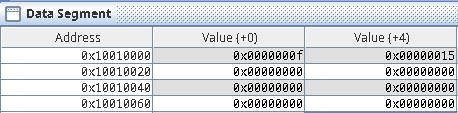
\includegraphics[width=.6\linewidth]{img/c1-1}
    \caption{Datos del programa según se indican en el panel de datos}
    \label{fig:c1-1}
\end{figure}

\subsection*{1.3}

De acuerdo a lo dicho en la teoría, las etiquetas \texttt{palabra1} y \texttt{palabra2} deberían tomar el valor de las posiciones de memoria a las que hacen referencia. En este caso, las ya mencionadas \texttt{0x1001000} y \texttt{0x00000015}, respectivamente.

\subsection*{1.4}

Al ensamblar el programa dado, no parece presentar ninguna diferencia con respecto al primer programa visto, ya sea tanto en la memoria, como también en otras variables visibles en el simulador (por ejemplo, los registros).

\subsection*{1.5}

El siguiente código cumple con la consigna planteada:

\vspace{7pt}
\usemintedstyle{murphy}
\inputminted[linenos]{gas}{src/cuestiones/c1-5.asm}
\vspace{7pt}

Y en la Figura \ref{fig:arr5-mem} podemos comprobar que los valores fueron almacenados de forma correcta, considerando que los números 30 y 60 en decimal se corresponden con \texttt{0x0000001e} y \texttt{0x0000003c} respectivamente.

\begin{figure}[h]
    \centering
    \captionsetup{justification = centering}
    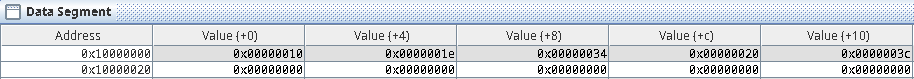
\includegraphics[width=.95\linewidth]{img/c1-5a}
    \caption{Valores del vector de números declarado en el programa propuesto, según se indican en el panel de datos}
    \label{fig:arr5-mem}
\end{figure}

Notar que al haber cambiado la dirección de memoria inicial donde se quiere que se almacenen los datos (respecto a la utilizada por defecto), debimos de expandir el panel de datos del simulador para poder visualizar el segmento de la memoria donde se ubicaban los valores reservados de nuestro vector, seleccionando la opción correspondiente desde un menú desplegable, tal como se lo muestra en la Figura \ref{fig:dropdown-data}.


\begin{figure}[h]
    \centering
    \captionsetup{justification = centering}
    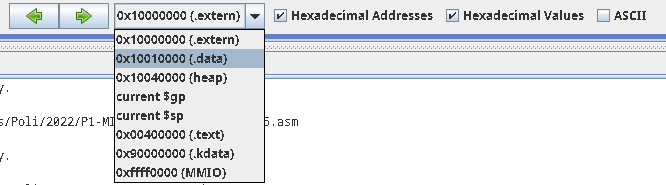
\includegraphics[width=.7\linewidth]{img/c1-5b}
    \caption{Menú desplegable para seleccionar la visualización del segmento de memoria correspondiente al utilizado por el programa planteado}
    \label{fig:dropdown-data}
\end{figure}

\subsection*{1.6}

Podemos probar cambiar el argumento de la directiva \mintinline{gas}{.data} para intentar almacenar los datos partiendo desde la dirección \texttt{0x10000002}:

\vspace{7pt}
\usemintedstyle{murphy}
\inputminted[linenos]{gas}{src/cuestiones/c1-6.asm}
\vspace{7pt}

Hecho este cambio, el panel de datos nos muestra que los valores ahora son almacenados partiendo desde la dirección de memoria \texttt{0x10000004}, saltando de 4 en 4 (por el tamaño de palabra, Fig. \ref{fig:not-multiple}).

\begin{figure}[ht!]
    \centering
    \captionsetup{justification = centering}
    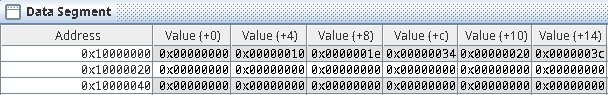
\includegraphics[width=.7\linewidth]{img/c1-6}
    \caption{Valores y respectivas posiciones de memoria del programa con argumento de \mintinline{gas}{.data} modificado}
    \label{fig:not-multiple}
\end{figure}

Esto difiere en principio de lo que uno podría esperar, ya que se le está indicando al ensamblador que ubique la información partiendo desde la dirección de memoria \texttt{0x10000002}. El motivo por el cual ejecuta el cambio descripto, es porque se requiere que la ubicación de todos los valores se encuentren en posiciones múltiplos de 4, de forma que la memoria ``esté alineada''. Éste es un requisito de la arquitectura MIPS, o bueno, al menos estamos seguros basándonos en lo visto en la teoría, que lo es para el lenguaje de máquina de los microprocesadores MIPS R2000.

Con esto en cuenta, el ensamblador, sabiendo que indicamos el espacio para datos partiendo desde la posición de memoria \texttt{0x10000002}, buscó por la posición de memoria (mayor o igual) múltiplo de 4 más cercana, y a partir de allí ubico los valores del vector de números reservado en el programa.

\end{document}
